%************************************************
\section*{Methodology}\label{ch:methodology}
%************************************************

\subsection*{Research Questions}\label{sec:research_questions}

\textbf{RQ1: How do commits interact with features structurally?}

We intend to research two main properties which already provide a lot of insight into the development process of features and usage of commits therein.
Firstly, we examine the amount of commits, features interact with structurally.
This gives us a direct estimate on how many commits were used in the development of a feature.
Our analysis also allows us to meausre the scope of feature
, which can put the amount of commits used to implement a feature into perspective.
Secondly, we want to examine how many features a commit interacts with structurally, e.g. how many features a commit usually changes. 
This is especially interesting when considering best practices surrounding the usage of commits.
It is preferred to keep commits granular meaning they should only fix a single bug or, in our case, change a single feature.
Acquiring data on this issue might show how strictly this policy is enforced in the development of features. \\

\begin{center}
\begin{tabular}{cc}
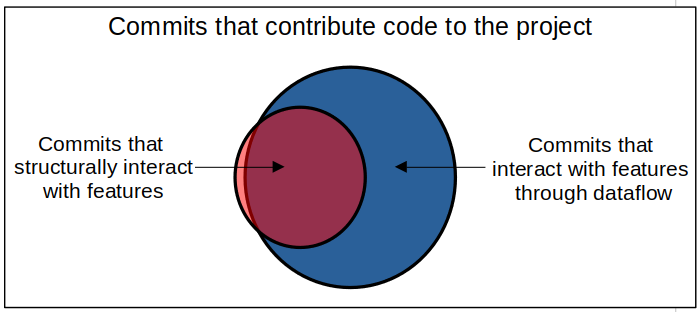
\includegraphics[height=6cm]{gfx/Commits-of-a-Software-Project.png}
\end{tabular}
\captionof{figure}{Kinds of Commits in a Software Project investigated in this work}
\end{center}

\textbf{RQ2: How do commits interact with features through dataflow?}

Investigating dataflow can unveil interactions between parts of a program that were previously hidden from programmers.
This can help a programmer understand the extend to which new changes affect other parts of a program.
Deploying the introduced analysis in an ad-hoc, functional manner could even aid a programmer when fixing bugs.
Bugs occuring in certain parts of a program could be traced back to their cause by factoring in recent changes affecting said parts through dataflow. \\
Previous research has laid the groundwork for researching dataflow interactions between different parts of a program.
However, it has focused solely on dataflow interactions between commits.
That's why we want to provide first insights on the properties of dataflow-based commit-feature interactions.
Specifically, we investigate how connected commits and features are by analyzing the amount of features a commit usually affects through dataflow.
Knowing what fraction of all commits contributing code to a project are part of dataflow-based interactions can show how often new commits affect the data of a feature. 
Regarding this, it is worth considering that commits constituting code of a feature are very likely to influence said feature through dataflow.
Since dataflow interactions coinciding with structural interactions are so obvious, programmers are also much more aware of them. 
Depending on the prevalence of feature-regions in a project's code space, this could heavily skew the data in one direction, as a large portion of all dataflow interactions would stem from these obvious interactions. 
Therefore we want to especially focus on commits that aren't part of a feature giving us more valuable and insightful information. \\

In the first two \textbf{RQs} we have discussed different kinds of commits and the ways in which they interact with features. 
Figure 1 showcases them in a venn diagram and illustrates the dependencies and divisions between them. \\

\textbf{RQ3: How do authors implement features?}

Usually there are many programmers working on the same software project, implementing different features, sometimes alone, sometimes with the help of colleagues.
We want to shine some light on the exact statistics of this by combining structural commit-feature interactions with high-level repository information.
One major question we want to answer is how many authors implement a feature on average, where considering feature-scope could help put this data into perspective.
Additionally we aim to investigate the extend to which each developer contributes to the implementation of a feature. 
This way we can detect development patterns like the existence of a main developer as discussed by \citet{sattler2023seal}. 
The collected results could serve as advice for software companies on how to allocate programmers on to-be implemented features. 

\subsection*{Operationalization}\label{sec:operationalization}

\textbf{RQ1: What are the characteristics of structural commit-feature interactions?}

The needed data will be collected by creating reports comprimising all structural commit-feature interactions of a chosen software project.
The collected data is then evaluated by iterating over all found commit-feature interactions.
For each encountered feature we save the commits it interacts with.
As the analysis has also calculated the amount of instructions a structural interaction occurs in 
we save the entire amount of such instructions for every feature.
We have previously noted that a feature only structurally interacts with a commit that has contributed code to said feature.
Besides that each line of code in a git project was added or changed by a commit, 
which means that each line of code that belongs to a feature also belongs to a commit.
Therefore the commits saved inside the interactions of a feature are the commits that constitue the code space of a feature. 
With this data, it's possible to calculate the average amount of commits used to create a feature, 
while being able to correlate this with its size, in our case, its number of instructions.
For the evaluation of the second point, we iterate over all found structural commit-feature interactions again, 
but instead save the features each encountered commit interacts with. 
From aforementioned explanations, it follows that a commit contributes code, e.g. implements, the feature it structurally interacts with. \\ 

\textbf{RQ2: How do commits interact with features through dataflow?}

The projects investigated for dataflow-based commit-feature interactions will be the same projects investigated for structural commit-feature interactions.
This choice will allow more insight into a single project and allow us to combine both analysis results as will be discussed below.
In \textbf{RQ2} we consider all commits that currently contribute code to the project, 
which we can extract from high level repository information of the project.
For each commit we will save whether and if true which features they interact with through dataflow.
Similarly to \textbf{RQ1}, this is carried out by iterating over the dataflow-based commit-feature interactions in the created reports.
The acquired information makes it possible to calculate what fraction of commits interact with features through dataflow.
For commits that do have dataflow-based interactions with features, we will examine how many features they interact with on average.
The dicussed separation for said commits into those that are part of a feature and those that aren't 
is accomplished with the usage of already created structural reports. 
We can find out whether a commit is part of a feature by checking if it is part of a structural commit-feature interaction in the according report. \\

\textbf{RQ3: How do authors implement features?}

Here, we will examine the same projects as the previous \textbf{RQs}.
That way we can reuse data produced in \textbf{RQ1} to map each feature to the authors that implemented it.
In \textbf{RQ1} we have already mapped each feature to the commits it interacts with, e.g. that contribute code to it.
It's possible to retract the authors of these commits by searching through high-level repository information with their hashes.
This will directly give us the authors that implemented a feature.
The amount of instructions that stem from code belonging to a feature has also been calculated for \textbf{RQ1}.
With this information we can correlate the size of a feature with the amount of developers that implemented it.
Furthermore we want to estimate the amount of code a developer contributes to a feature.
To accomplish this, we adapt the analysis used to map each feature to the authors that implement them.
When iterating over the commit-feature interactions we not only save the commit, but addtionally save the amount of instructions of that interaction.
When extracting the authors from the commits that were mapped to a feature, we also add up the amount of instructions for each commit.
Now we can estimate the amount of code an author contributes to a feature with the amount of instructions stemming from said code.

\subsection*{Expectations}\label{sec:expectations}

How and to which extend features are used in the projects to be examined is not known and could potentially vary from project to project.
Thus, some results of the dicussed research topics are difficult to predict.
For example, nesting of feature regions inside each other could lead to an increase in the amount of features a commit usually changes.
Due to the discussed best practices of commits, we expect commits to change at most one feature on average if there happens to be little nesting.
Because of the unknown size of features, it's not sensible to give an estimate about the amount of commits needed to implement a feature.
We expect a rather strong positive correlation between the scope of a feature and its commits however.
It was mentioned that we examine small projects meaning that the pool of developers is limited in size. 
Normally, features only encompass a tiny share of a project's overall code. 
Besides that they implement specific functionality that some programmer's might have a better understanding of than others.
This leads us to the expectation that a feature is implemented by a small share of all developers contributing to a project.
Because of the small pool of developers and prior research findings, we expect the existence of a main developer that contributes most if not all of the functionality of a feature.
We know that commits structurally interacting with features most likely are part of dataflow interactions with them as well.
Excluding such commits, the extend to which commits interact with features through dataflow depends heavily on what fraction of the code space is made up of feature regions.
The purpose of features is to implement additional and sometimes necessary functionality separate from the main program.
For this they access and change specific data according to their intended functionality.
Provided that feature regions only make up a small portion of the program, we do expect relatively few, albeit important dataflow interactions between commits and features.

\subsection*{Threats to Validity}\label{sec:threats}

There are some potential threats to the internal validity of our gathered data, which stem from our implementation in VaRA. \\
From \textbf{Definition 2} of feature regions, it follows that we implement feature regions in such a way that any instruction whose execution depends on a configuration variable, is part of a feature region.
However, not every such instruction also implements the functionality of a feature, meaning that feature regions overapproximate the amount of instructions responsible for a feature's functionality.
Since feature regions are used for computing both structural and dataflow-based commit-feature interactions, they are overapproximated to some extend as well.
Thus, it's possible that commits of structural interactions don't actually implement functionality of a feature and commits of dataflow interactions don't actually affect instructions implementing a feature's functionality through dataflow.
Furthermore our deployed taint analysis does not necessarily detect all dataflows occuring in a program.
This results in taints being underapproximated, meaning that some instructions are not tainted when they correctly should be.
Thus, some dataflow interactions could be missed by our deployed commit-feature interaction detection. \\
Concerning the external validity of our findings, most dangers come from the selection of which projects we investigate.
In previous chapters we have discussed that the chosen projects are rather small and are of a ... domain.
This could mean that our findings might not be applicable for projects of larger size or of different domains.
As we already factor in the scope of a feature in the analysis of our data, we are able mitigate some doubts about the applicability of our results onto larger projects.



